\subsection*{Part A}
\begin{enumerate}
    \item Navigate to the Windows Firewall menu through the System and Security settings in the Windows Control Panel.
    \begin{figure}[H]
        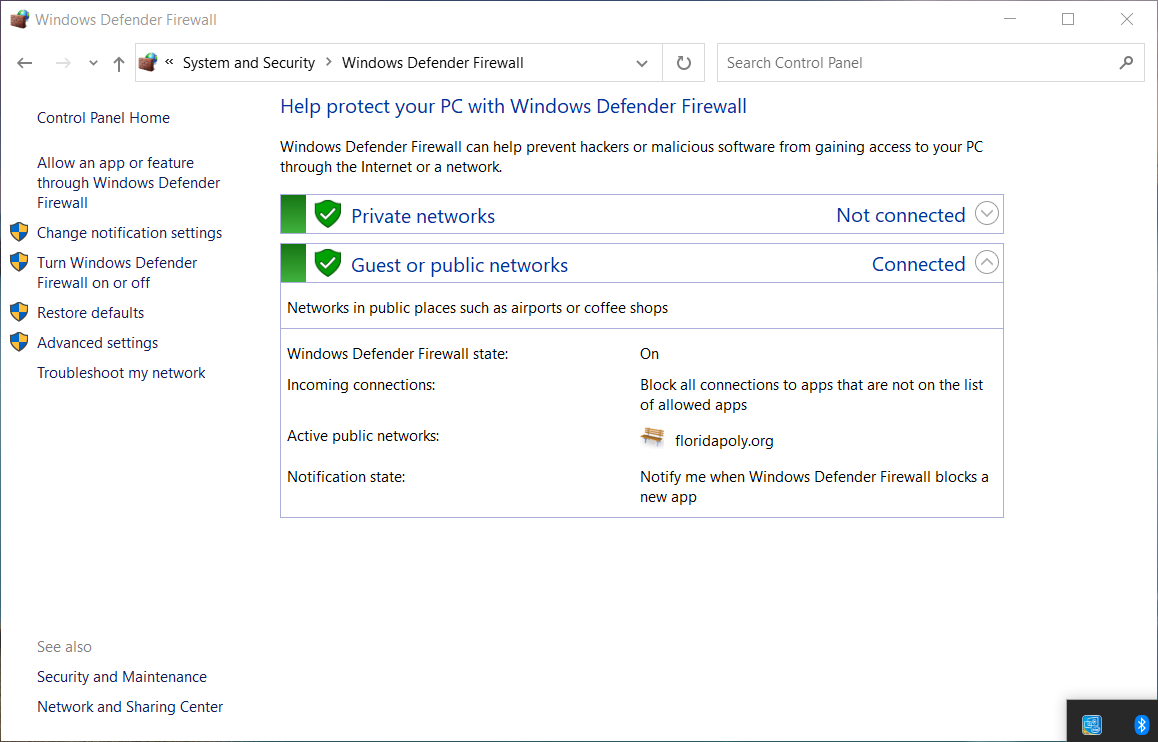
\includegraphics[width=\linewidth]{figures/pic1.png}
    \end{figure}
    \item The Windows Firewall is active for both the \textbf{public} and \textbf{private} networks.
    \item All incoming connections are disabled (including allowed programs) to avoid malicious incoming connections on public networks.
    \begin{figure}[H]
        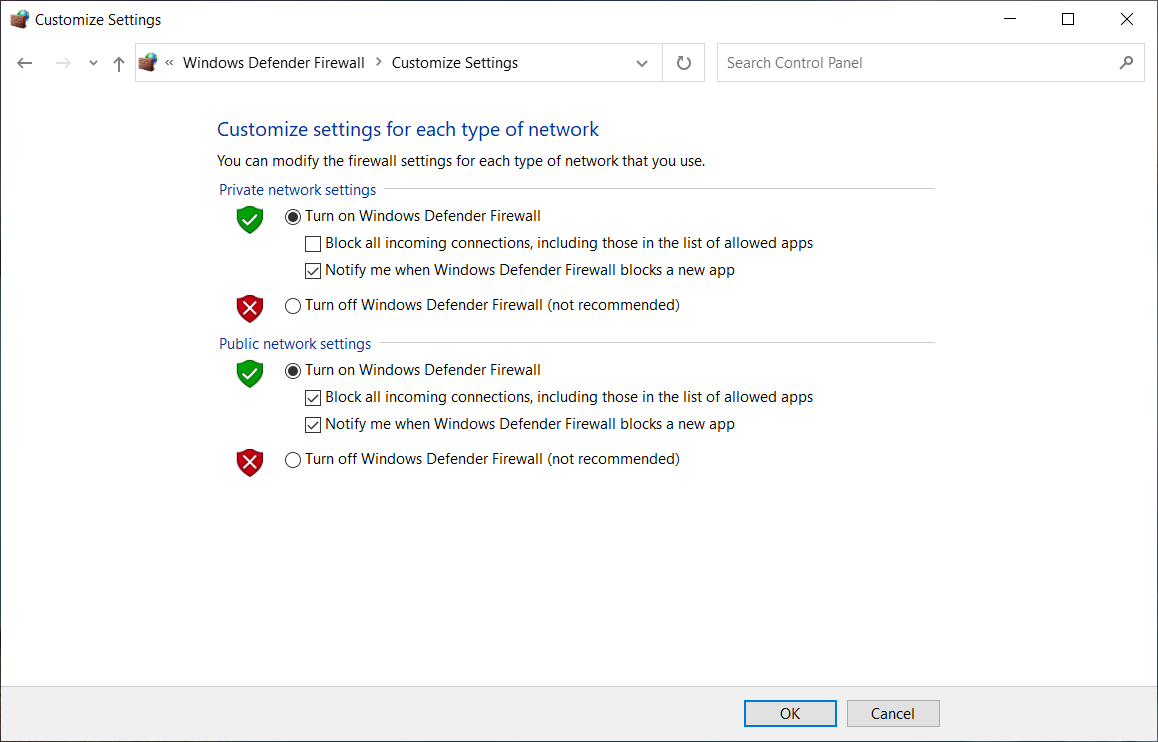
\includegraphics[width=\linewidth]{figures/pic2.png}
    \end{figure}
    \item In order for applications to bypass the firewall, they have to be allowed in the firewalls \textbf{Allowed Apps}
    \item Each program can be allowed through the public, private or both networks.
    \item We do not allow any apps to bypass the public firewall because this is a security risk.
    \begin{figure}[H]
        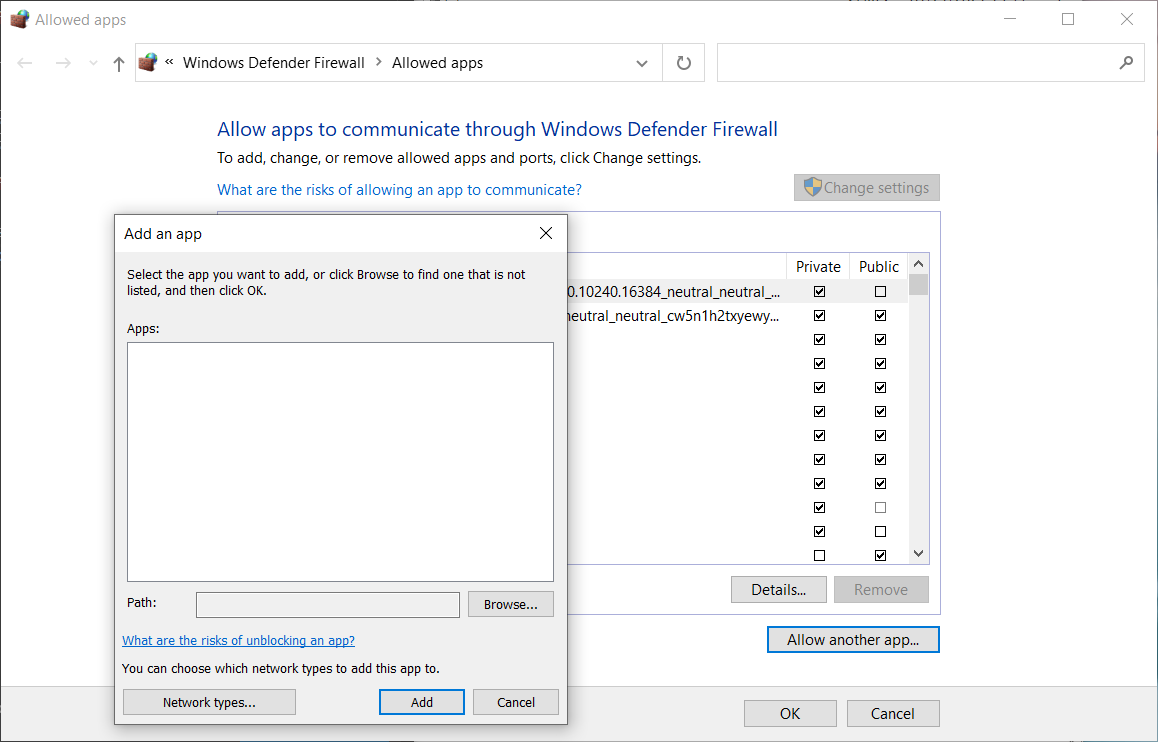
\includegraphics[width=\linewidth]{figures/pic8.png}
    \end{figure}
    \item Navigate to the \textbf{Advanced Settings} to further examine the properties of the Windows firewall.
    \item Navigate to the \textbf{Windows Firewall Properties}
    \item Viewing the settings for each of the Domain, Public and Private profiles, the Public profile has the property: \textbf{Block all connections} under the \textbf{Inbound Connections} setting because this setting was altered in step 3.
    \begin{figure}[H]
        \begin{subfigure}[b]{0.3\textwidth}
            \centering
            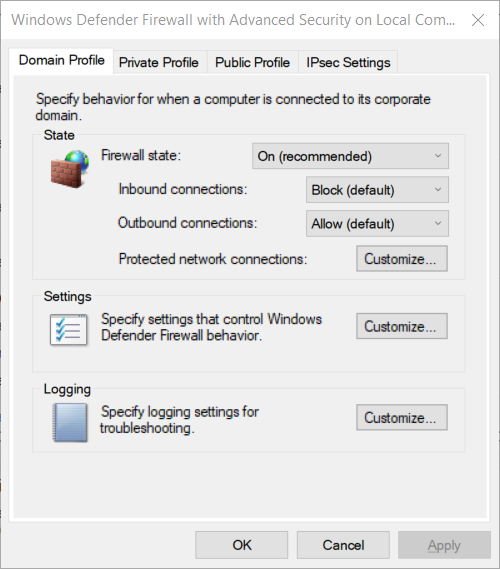
\includegraphics[width=\textwidth]{figures/pic5.png}
        \end{subfigure}
        \begin{subfigure}[b]{0.3\textwidth}
            \centering
            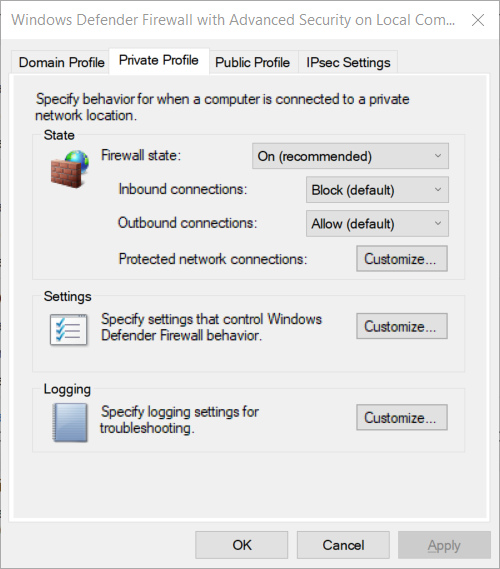
\includegraphics[width=\textwidth]{figures/pic6.png}
        \end{subfigure}
        \begin{subfigure}[b]{0.3\textwidth}
            \centering
            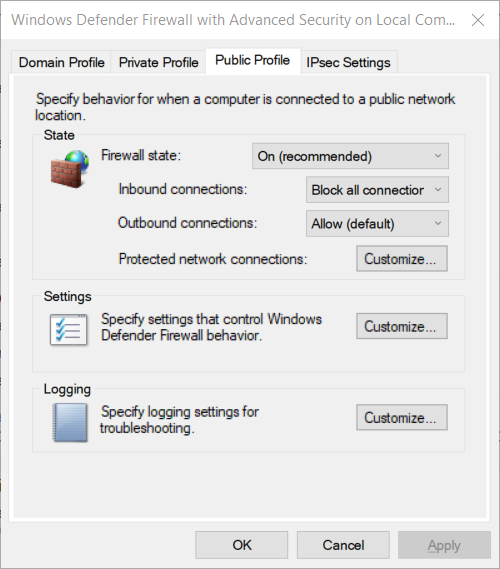
\includegraphics[width=\textwidth]{figures/pic7.png}
        \end{subfigure}
    \end{figure}
    \item Having the \textbf{Display a notification} enabled when a program is blocked by the firewall is important so that the user has the knowledge that a program was trying to gain access, allowing them to take the necessary actions.
    \item Now we return to the Windows firewall advanced security page.
\end{enumerate}

